\section{Introduction}
\label{leffa:sec:introduction}

Controllable person image generation aims to generate an image of a person guided by reference images, allowing for control over attributes such as appearance and pose.
Underpinning a wide variety of applications in virtual and augmented reality, gaming, and e-commerce, this task has made significant progress~\citep{kim2024stableviton, choi2024improving, chong2024catvton, wan2024improving, bhunia2023person, han2023controllable, lu2024coarse, pham2024cross} based on the advancements in diffusion-based image generation~\citep{ho2020denoising, rombach2022high}.

The primary challenge in this task is to preserve the \textit{fine-grained details} (\eg, textures, texts, logos, \etc) from the reference image while maintaining \textit{overall quality}.
Although current methods can generate high-quality images at first glance, they still suffer from the distortion of fine-grained textural details upon closer inspection (see Fig.~\ref{subfig:intro_2} top, where the striped texture is wrong).
Researchers have attempted to improve the preservation of fine-grained details by integrating inference strategies (\eg, disentangled guidance~\citep{bhunia2023person}, multi-stage inference~\citep{yang2024texture}, incorporating information from other modalities~\citep{ning2024picture, xu2024ootdiffusion, choi2024improving} (\eg, textual descriptions) and introducing auxiliary models for feature improvement~\citep{kim2024stableviton, xu2024ootdiffusion, choi2024improving, wan2024improving, sun2024outfitanyone, lu2024coarse, pham2024cross} (\eg, using CLIP~\citep{radford2021learning}, DINOv2~\citep{oquab2023dinov2} features, and warping model, \etc).
However, these methods typically increase model complexity and lack \textit{explicit} supervision to establish visual consistencies between the target and reference images.

By visualizing the attention layer of various diffusion-based methods~\citep{choi2024improving, xu2024ootdiffusion}, we observe that in regions where details are distorted, the target query exhibits \textit{widely-distributed} attention rather than accurately focusing on the corresponding reference key regions.
This observation also aligns with findings from previous studies~\citep{kim2024stableviton, ren2022neural}.
For instance, in Fig.~\ref{subfig:intro_2}, the incorrect generation of striped texture results from the target query failing to attend to the corresponding reference key regions.
In contrast, when the attention map is \textit{manually corrected} by swapping the highest-response values with those lying in the correct region, the model is able to generate significantly improved striped textures without any additional training (see Fig.~\ref{subfig:intro_3}).

Capitalizing on this observation, we propose a regularization loss by \textbf{le}arning \textbf{f}low \textbf{f}ields in \textbf{a}ttention (\textbf{\leffa{}}) to alleviate the distortion of fine-grained details.
Specifically, we transform the attention map between the target query and reference key into a flow field during training, which warps the reference image to more closely align with the target image. This process encourages the target query to accurately attend to the correct reference key.

To validate our method, we incorporate our \leffa{} loss into a diffusion-based baseline, observing a significant reduction in fine-grained detail distortion while maintaining high image quality (see Fig.~\ref{subfig:intro_4} top), without additional inference cost.
Additionally, visualization of our method's attention map (see Fig.~\ref{subfig:intro_4} bottom) confirms the model accurately focuses on the desired regions.
We quantitatively and qualitatively evaluate our method on virtual try-on (appearance control) with VITON-HD~\citep{choi2021viton} and DressCode~\citep{morelli2022dress}; and pose transfer (pose control) with DeepFashion~\citep{liu2016deepfashion}, both achieving state-of-the-art performance and mitigating the distortion of fine-grained details across all datasets.
Finally, we show that our \leffa{} loss is model-agnostic and generalizes effectively to other diffusion-based methods~\citep{choi2024improving, chong2024catvton}, demonstrating \leffa{} as a versatile and general solution for controllable person image generation.

The contributions of this chapter are as follows:
\begin{itemize}
    \item We propose \leffa{}, a regularization loss that explicitly guides the target queries in attention layers to focus on correct reference keys, mitigating detail distortion without additional parameters and inference cost. 
    \item We evaluate \leffa{} on both virtual try-on and pose transfer across various diffusion-based methods, achieving state-of-the-art quantitative performance and significantly reducing fine-grained detail distortion qualitatively.
\end{itemize}


\begin{figure}[t!]
    \centering
    \caption{
    Taking appearance control of a person image (virtual try-on) as an example:
    (a) input person and reference (garment) images;
    (b) generated image and attention map from a diffusion-based method (\eg, IDM-VTON~\citep{choi2024improving});
    (c) generated image after \textit{manually modifying} the attention map in the diffusion-based method to focus on the correct regions;
    (d) generated image and attention map from \leffa{}.
    Our method generates high-quality images without detail distortion (see the colored striped texture).
    }
    \begin{subfigure}[t]{0.249\linewidth}
        \centering
      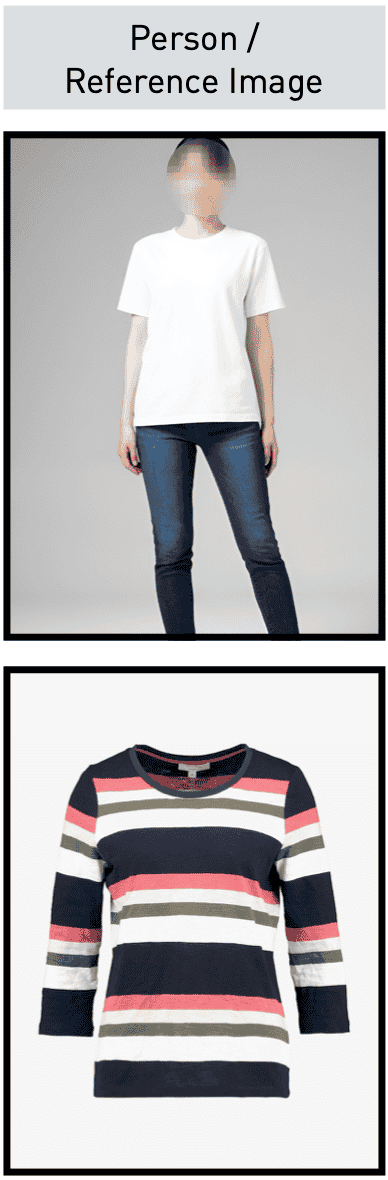
\includegraphics[width=\linewidth]{Chapter6/Figures/intro_1_final-min.png}
      \caption{}
        \label{subfig:intro_1}
    \end{subfigure}\hfill
        \begin{subfigure}[t]{0.249\linewidth}
        \centering
          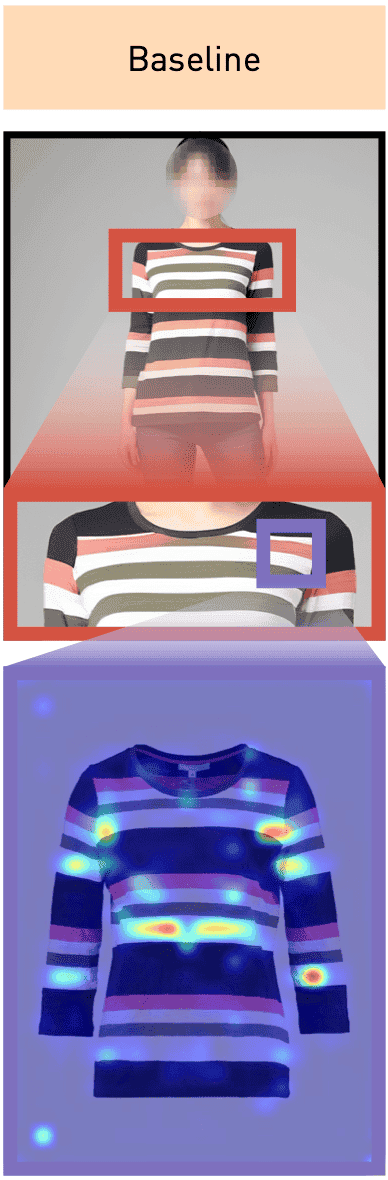
\includegraphics[width=\linewidth]{Chapter6/Figures/intro_2_final-min.png}
              \caption{}
        \label{subfig:intro_2}
    \end{subfigure}\hfill
        \begin{subfigure}[t]{0.249\linewidth}
        \centering
          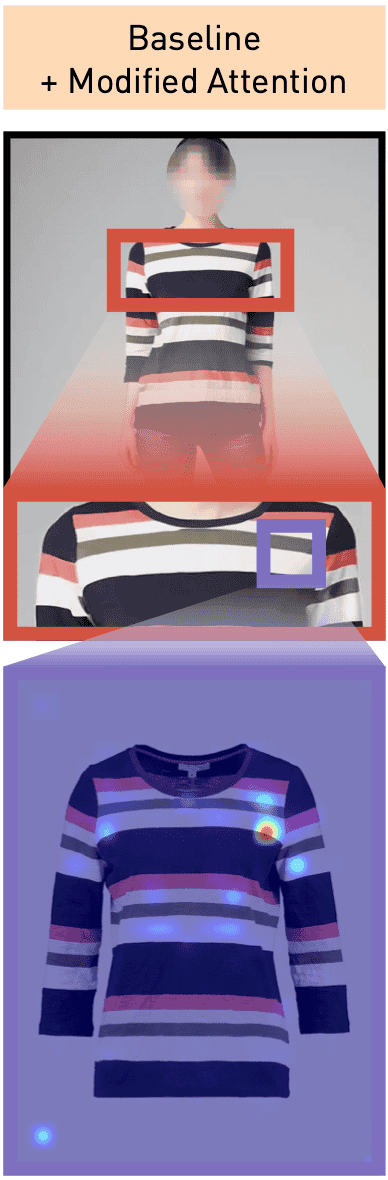
\includegraphics[width=\linewidth]{Chapter6/Figures/intro_3_final-min.png}
                \caption{}
        \label{subfig:intro_3}
    \end{subfigure}\hfill
        \begin{subfigure}[t]{0.249\linewidth}
        \centering
        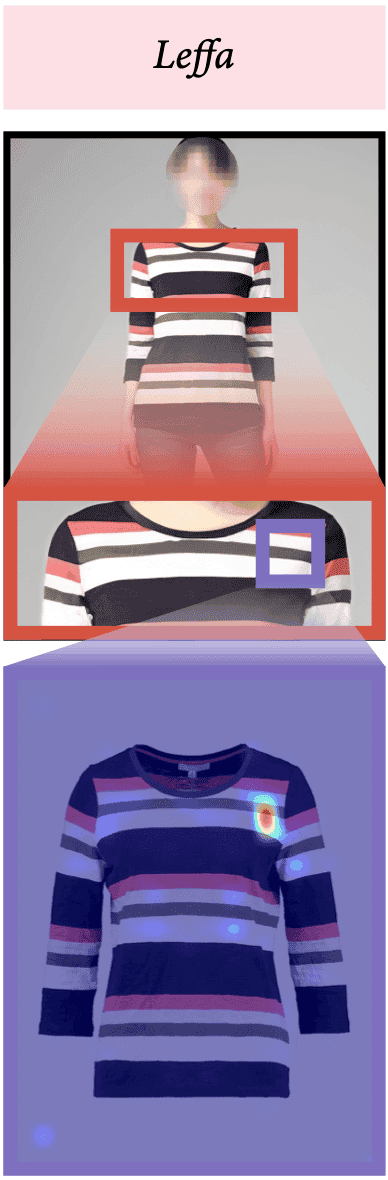
\includegraphics[width=\linewidth]{Chapter6/Figures/intro_4_final-min.png}
        \caption{}
        \label{subfig:intro_4}
    \end{subfigure}
    \label{leffa:fig:introduction}
\end{figure}


